\documentclass[bibliography=totocnumbered]{scrartcl}

% Codificación
\usepackage[utf8]{inputenc}
% Idioma
\usepackage[spanish]{babel}
% Bibliografía
\usepackage{csquotes}
\usepackage[backend=biber,citestyle=numeric,dateabbrev=false,language=spanish,sorting=nty]{biblatex}
\addbibresource{./referencias.bib}
% Links
\usepackage{hyperref}
\hypersetup{
    colorlinks=true,
    citecolor=black,
    filecolor=black,
    linkcolor=black,
    urlcolor=black
}
% Código de programación
\usepackage{listings}
% SetUp de colores para código
\usepackage{xcolor}
\definecolor{codegreen}{rgb}{0,0.6,0}
\definecolor{codegray}{rgb}{0.5,0.5,0.5}
\definecolor{codepurple}{rgb}{0.58,0,0.82}
\definecolor{backcolour}{rgb}{0.95,0.95,0.92}
\lstdefinestyle{mystyle}{
    %backgroundcolor=\color{backcolour},   
    commentstyle=\color{codegreen},
    keywordstyle=\color{magenta},
    numberstyle=\tiny\color{codegray},
    stringstyle=\color{codepurple},
    basicstyle=\ttfamily\footnotesize,
    breakatwhitespace=false,         
    breaklines=true,                 
    captionpos=b,                    
    keepspaces=true,                 
    %numbers=left,                    
    numbersep=5pt,                  
    showspaces=false,                
    showstringspaces=false,
    showtabs=false,                  
    tabsize=2
}
\lstset{style=mystyle}
% Imágenes
\usepackage{graphicx}
% Cambios de color para links
\newcommand{\changeurlcolor}[1]{\hypersetup{urlcolor=#1}} 
\title{Cross-site Scripting (XSS)}
%\subtitle{subtitle}
\author{Víctor Nieves Sánchez}
\date{Última modificación \today{}}

\begin{document}
\maketitle
\section*{Disclaimer}
Este documento se ha elaborado por los autores, obteniendo información de diversos recursos, principalmente de la página web de \changeurlcolor{blue}\href{https://portswigger.net/web-security}{\textit{PortSwigger}}.\\
\changeurlcolor{black}
El objetivo de este documento es proporcionar una breve referencia de ayuda para el lector.\\

Si deseas más información, os recomendamos realizar los labs de su página web:
\begin{center}
\changeurlcolor{blue}\href{https://portswigger.net/web-security}{https://portswigger.net/web-security}    
\end{center}

\newpage
\tableofcontents

\newpage
\listoffigures

\newpage

\section{¿Qué es Cross-site scripting?}
\textit{Cross-site scripting} conocido como \textit{XSS}, es un tipo de vulnerabilidad web que permite al atacante comprometer la interacción de los usuarios con la aplicación. Esta vulnerabilidad normalmente permite al atacante hacerse pasar por la víctima, para llevar acabo cualquier acción que ésta pueda hacer, dándole acceso a la información del usuario. Si el usuario tiene privilegios de acceso en la aplicación, entonces el atacante podría ser capaz de hacerse con el control de la aplicación (funcionalidad y datos).

\section{¿Cómo funciona el XSS?}
Funciona manipulando una web vulnerable para que esta retorne código \textit{JavaScript} malicioso a los usuarios. Cuando este código se ejecuta en el buscador de una víctima, el atacante podrá comprometer la interacción de la víctima.
\begin{figure}[h]
  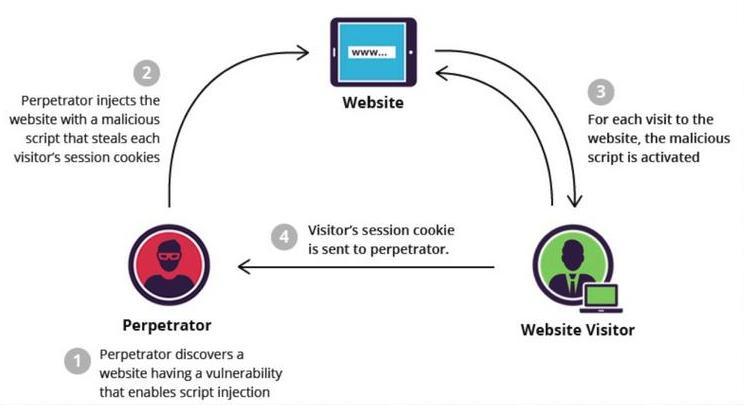
\includegraphics[width=\linewidth]{figures/xssStored.jpg}
  \caption{Funcionamiento de XSS}
  \label{fig:XssStored}
\end{figure}

\section{Tipos de XSS?}
\subsection{XSS reflejado \textit{(Reflected XSS)}}

\subsection{XSS almacenado \textit{(Stored XSS)}}

\subsection{XSS basado en DOM \textit{(DOM-based XSS)}}


\newpage
% Citar todas las ref (incluidas las que no han sido citadas)
\nocite{*}
\printbibliography 
\end{document}




